
\section{LANDSCAPE} \label{landscape}

The online digital files market is rapidly expanding and as we can see in Figure \ref{fig:market}, it is expected to double in size over the next two years. Among the types of files that are sold online, Ebooks and music account for over 50\% of the sales ( Figure \ref{fig:file_categories} ). 
As the market expands, a multitude of distribution channels exist for creators to sell their digital content. The main distinction among current offerings is whether the solution used facilitates a direct connection between the creator and the buyer or it enables the creator to reach a wider audience without facilitating a direct sell. Using industry terms, the two main offerings are known as Maker Platforms and Exchange Platforms and in the following section we will review their advantages and shortcomings. 

\begin{figure}[b]
\centering
\begin{minipage}{.5\textwidth}
  \centering
  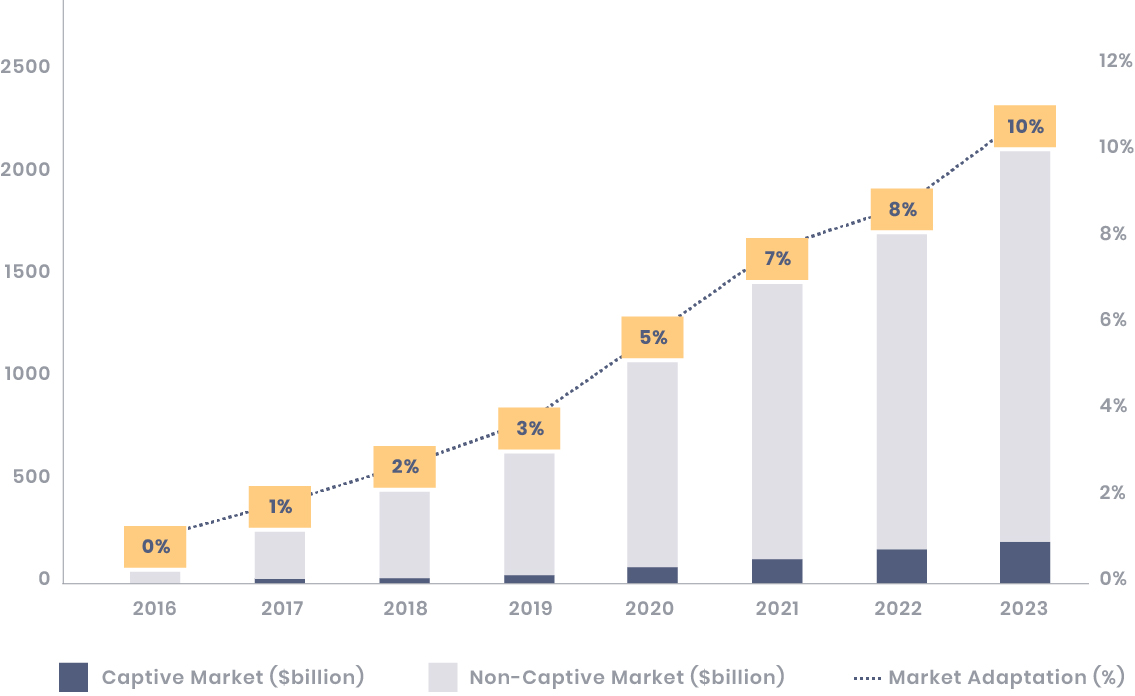
\includegraphics[width=0.8\linewidth]{./figures/fig1.jpg}
  \captionof{figure}{Online digital files market ( \$billion )}
  \label{fig:market}
\end{minipage}%
\begin{minipage}{.5\textwidth}
  \centering
  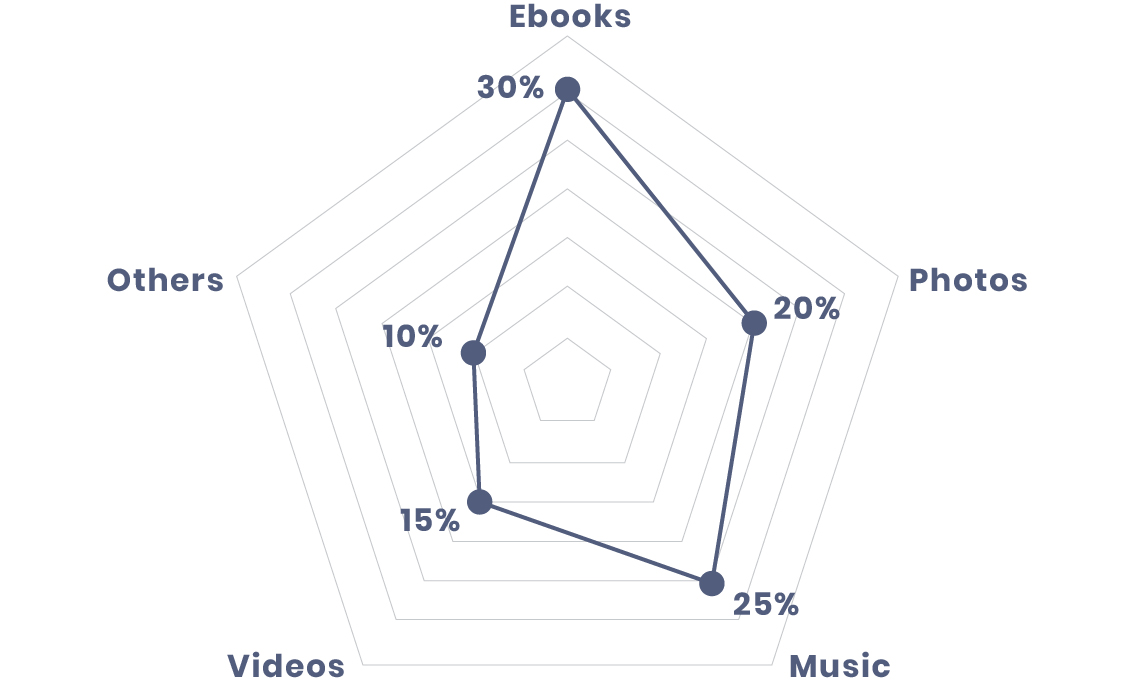
\includegraphics[width=0.8\linewidth]{./figures/fig2.jpg}
  \captionof{figure}{Digital file categories sales}
  \label{fig:file_categories}
\end{minipage} 
\end{figure}


%%%%%%%%%%%%%%%%%%%%%%%%%%%%%%%%%%%%%%%%%%%%%%%%%%%%%%%%%%%%%%%%%%%%%%
\subsection{Maker Platforms}

Several stock content websites exist where creators can fully give up their licensing and pricing rights and get a commission on copies of work sold. Such websites do not require a subscription by the creator but are customer centric and provide subscription plans for end users. Submitted work needs to go through a thorough vetting process before it is included in the catalog of works available. Such websites theoretically offer a lot of visibility since they tend to have a huge user base but, in practice, ones work can easily be lost among the myriad of similar offerings. As we can see in Table \ref{comp-matrix} creators only receive a small fraction of the retail price of their work, buyers need to have a valid paid subscription and creators have no control over the licensing and pricing of their work.


% Please add the following required packages to your document preamble:
% \usepackage{booktabs}
\begin{table}[t]
\centering
\begin{tabular}{@{}rlll@{}}
\toprule
\multicolumn{1}{l}{}         & \multicolumn{1}{c}{\textbf{Maker Platforms}} & \multicolumn{1}{c}{\textbf{Exchange Platforms}} & \multicolumn{1}{c}{\textbf{BlockLicense}} \\ \midrule
\textbf{Targetting}          & Buyers                                       & Creators                                        & Creators \& Buyers                        \\
\textbf{License Issuer}      & Service Provider                             & Creators                                        & Creators                                  \\
\textbf{Pricing}             & Service Provider                             & Creators                                        & Creators                                  \\
\textbf{Uncapped Files}      & No                                           & No                                              & Yes                                       \\
\textbf{Creator Branding}    & No                                           & Yes                                             & Yes                                       \\
\textbf{Subscription Fees}   & Yes                                          & Yes                                             & No                                        \\
\textbf{Instant Payouts}     & No                                           & No                                              & Yes                                       \\
\textbf{Central Web Market}  & Yes                                          & Some                                              & Yes                                       \\
\textbf{Website Embedded Shop}	& No                                           & Yes                                             & Yes                                       \\
\textbf{Crypto Transactions} & No                                           & Some                                              & Yes                                       \\
\textbf{Sales Fees}          & 65\% - 85\%                                  & 2.9\% - 10\%                                    & 2\%                                       \\ \bottomrule
\end{tabular}
\caption{Feature comparison matrix}
\label{comp-matrix}
\end{table}



%%%%%%%%%%%%%%%%%%%%%%%%%%%%%%%%%%%%%%%%%%%%%%%%%%%%%%%%%%%%%%%%%%%%%%

\subsection{Exchange Platforms}

Exchange platforms enable creators to facilitate a direct sell by providing an inventory, payment processing, shopping cart and cloud based storage as a service. Such offerings usually require a time-based subscription by the creator and display product listings either in a central website or provide embeddable widgets that creators can use to display and sell their products through their own website. While Exchange Platforms give full control to creators over the licensing and pricing of their work, as we can see in Table \ref{comp-matrix} they are charged a fee on work sold and an active paid subscription is required.
\newline

In contrast to Maker \& Exchange platforms, BlockLicense doesn't require a subscription fee by creators or buyers, it allows creators to set their own licensing and pricing options for their work and only charges a 2\%  fee on work sold. In the following sections we will have a look at the types of licenses supported by BlockLicense and the types of licensing scenarios supported. The main distinction is whether the license corresponds to an open source license that is free to use or a commercial one that requires a fee.
